\chapter{كتابة نصوص باستعمال \textenglish{SDL\_ttf}}

يمكنني التكهّن بأن معظم القرّاء قد طرح هذا السؤال من قبل : "و لكن، ألا توجد أي دالة لكي تكتب نصاً على نافذة
\textenglish{SDL} ؟"
حان الوقت لأجيبك : الجواب هو لا.

رغم ذلك، توجد طرق لفعل هذا. يمكننا فقط \dots وضع صور للحروف بجانب بعضها البعض على الشاشة. هذا الأمر يعمل لكنّه ليس عمليا.

لحسن الحظ، يوجد ماهو أبسط : يمكننا استعمال المكتبة
\textenglish{SDL\_ttf}.
إنها مكتبة تتم إضافتها إلى الـ\textenglish{SDL}
تماماً مثل الـ\textenglish{SDL\_image}.
دورها هو إنشاء مساحة
\InlineCode{SDL\_Surface}
إنطلاقا من النص الذي نبعثه لها.

\section{تسطيب \textenglish{SDL\_ttf}}

يجب أن تعرف أنه، مثل
\textenglish{SDL\_image}، \textenglish{SDL\_ttf}
هي مكتبة تحتاج إلى أن تكون المكتبة
\textenglish{SDL}
مثبّتة من قبل. حسناً : إذا كنت إلى حدّ الآن لم تتمكّن من تسطيب المكتبة
\textenglish{SDL}
فهذا أمر شنيع و لهذا فسأعتبر أنك قمت بذلك !

تماما مثل 
\textenglish{SDL\_image}،
فإن المكتبة 
\textenglish{SDL\_ttf}
هي واحدة من المكتبات المُرتبطة بالـ\textenglish{SDL}
الأكثر شعبية (أي أنه يتم تنزيلها بكثرة). كما ستُلاحظ، هذه المكتبة مُبرمجة بشكل جيد. ما إن تجيد استعمالها لن يمكنك أن تتوقّف عن ذلك !

\subsection{كيف تعمل \textenglish{SDL\_ttf} ؟}

\textenglish{SDL\_ttf}
لا تقوم بإظهار صور 
\textenglish{bitmap}
لتولّد نصا في مساحات. في الحقيقة، هي طريقة ثقيلة لفعلها و لن يتاح لنا استعمال سوى خط واحد. \\
في الواقع، تستدعي المكتبة
\textenglish{SDL\_ttf}
مكتبةَ أخرى : 
\textenglish{FreeType}.
هي مكتبة قادرة على قراءة ملفات خطوط بصيغة
\InlineCode{.ttf}
لتُخرج منها صورة. تقوم
\textenglish{SDL\_ttf}
باسترجاع هذه الصورة و تحوّلها للـ\textenglish{SDL}
و ذلك بإنشاء مساحة
\InlineCode{SDL\_Surface}.

و بهذا فإن
\textenglish{SDL\_ttf}
تحتاج المكتبة
\textenglish{FreeType}
لكي تشتغل، و إلا فلن تكون قادرة على قراءة ملفات الخطوط
\InlineCode{.ttf}.

إذا كنت تعمل بـ\textbf{\textenglish{Windows}}
و تستعمل، مثلما أفعل، النسخة المُترجمَة للمكتبة، لن تحتاج إلى تنزيل أي شيء لأن
\textenglish{FreeType}
مضمّنة من قبل في المكتبة الحيّة
\InlineCode{SDL\_ttf.dll}
و لهذا فليس عليك القيام بأي شيء.

إذا كنت تعمل بالـ\textbf{\textenglish{GNU/Linux}}
أو
\textbf{\textenglish{Mac OS X}}
فمن اللازم أن تعيد ترجمة المكتبة، فتلزمك
\textenglish{FreeType}
لتتم الترجمة. اذهب إذن إلى صفحة تنزيل
\textenglish{FreeType} :

\url{http://www.freetype.org/download.html#stable}

لتنزيل الملفات الخاصة بالمطورين.

\subsection{تثبيت \textenglish{SDL\_ttf}}

اذهب إلى  صفحة تنزيل 
\textenglish{SDL\_ttf} :

\url{http://www.libsdl.org/projects/SDL_ttf/}

هنا، اختر الملف اللازم من القسم
"\textit{\textenglish{Binary}}".

\begin{information}
في
\textenglish{Windows}،
 لاحظ أنه لا يوجد سوى ملفان بصيغة 
\InlineCode{.zip}
يحملان في نهاية اسميهما اللاحقتين
\InlineCode{win32}
و
\InlineCode{VC6}.
الأولى 
(\InlineCode{win32})
تحتوي الـ\textenglish{DLL}
التي تحتاج إلى تقديمها مع الملف التنفيذي. يجب عليك أيضاً وضع هذه الـ\textenglish{DLL}
في مجلّد المشروع لتستطيع تجريب البرنامج، طبعا.

الثانية 
(\InlineCode{VC6})
تحتوي الملفات 
\InlineCode{.h}
و الملفات
\InlineCode{.lib}
التي تحتاجها للبرمجة. يمكننا أن نفكّر من خلال الاسم أن هذه الملفّات تخص
\textenglish{Visual C++}
فقط، لكن في الحقيقة، و بشكل خاص، الملف
\InlineCode{.lib}
يعمل أيضاً مع
\textenglish{mingw32}،
سيشتغل إذن في الـ\textenglish{Code::Blocks}.
\end{information}

الملف
\InlineCode{.zip}
يحتوي كالعادة مجلد
\InlineCode{include}
و مجلد
\InlineCode{lib}.
قم بوضع محتوى المجلد
\InlineCode{include}
في المسار
\InlineCode{mingw32/include/SDL}،
و محتوى المجلد
\InlineCode{lib}
في المسار 
\InlineCode{mingw32/lib}.

\begin{warning}
 يجدر بك نسخ الملف
\InlineCode{SDL\_ttf.h}
في المجلد
\InlineCode{mingw32/include/SDL}
و ليس في المجلد 
\InlineCode{mingw32/include}
فقط. احذر الخطأ !
\end{warning}

\subsection{تخصيص مشروع من أجل الـ\textenglish{SDL\_ttf}}

بقيت لنا مرحلة واحدة أخيرة : تخصيص المشروع لكي يكون قادراً على استعمال
\textenglish{SDL\_ttf}
بشكل جيد. يجب أن يتم التعديل على خصائص محرّر الروابط لكي يُترجم البرنامج بشكل جيد و ذلك باستعمال
\textenglish{SDL\_ttf}.

لقد تعلّمت من قبل هذه العملية بالنسبة لـ\textenglish{SDL\_image}،
و لهذا سأسرع قليلاً. \\
بما أنني أعمل في الـ\textenglish{Code::Blocks}
سأعطيك العملية الخاصة بهذه البيئة التطويرية. بالنسبة لباقي البيئات، فالطريقة لا تختلف كثيراً عن هذه :

\begin{itemize}
	\item توجّه نحو القائمة
	\InlineCode{Project} / \InlineCode{Build Options}.
	\item في القسم
	\InlineCode{Linker}
	أنقر على الزر الصغير
	\InlineCode{Add}.
	\item أشر إلى المسار الذي يوجد به الملف
	\InlineCode{SDL\_ttf.lib}
	(بالنسبة لي هو في\\
	\InlineCode{C:\textbackslash Program Files\textbackslash CodeBlocks\textbackslash mingw32\textbackslash lib}).
	\item ستظهر لك هذه الرسالة :
	"\textenglish{Keep this as a relative path ?}"
	لا يهمّ ما تختاره لأن الأمر سيشتغل في كلتا الحالتين. أنصحك أن تجيب بالسلب لأن المشروع لن يشتغل لو وضعته في مسار آخر غير المتواجد به لو أنك أجبت بالإيجاب.
	\item وافق على التغييرات بالنقر على 
	\InlineCode{OK}.
\end{itemize}

\begin{question}
ألا نحتاج إلى ربط المكتبة
\textenglish{FreeType}
أيضاً ؟
\end{question}

كلا، مثلما قلتُ فـ\textenglish{FreeType}
مضمّنة في الـ\textenglish{DLL}
الخاصة بـ\textenglish{SDL\_ttf}.
لهذا فلن يكون عليك الاهتمام بها، لأن
\textenglish{SDL\_ttf}
تفعل ذلك الآن.
\subsection{الملفات التوثيقية}

و الآن بما أنك أصبحت مبرمجاً محنّكاً تقريباً، يجدر بك أن تطرح التساؤل التالي : "لكن أين هو التوثيق ؟" إن لم تطرح هذا السؤال فهذا يعني أنّك لازلت لم تصبح بعد مبرمجاً محنّكاً.

يوجد بالطبع دروس تفصّل في كيفية عمل المكتبات، مثل هذا الكتاب، و لكن :

\begin{itemize}
	\item لن أستطيع أن أضع لك فصلاً حول كل المكتبات الموجودة (حتى لو أمضيت حياتي كلّها في ذلك، لن يكفيني الوقت !). و لهذا يجب عاجلاً أم آجلا قراءة التوثيق و يجدر بك أن تتعوّد على ذلك من الآن !
	\item من جهة أخرى، في غالب الأحيان تكون المكتبة معقّدة نوعاً ما و تحتوي كثيراً من الدوال. لن أتمكن من تقديم كلّ هذه الدوال في هذا الفصل لأنه سيكون بذلك طويلاً جداً !
\end{itemize}

من الواضح جداً أن التوثيق يكون كاملا و يلمّ بكل خفايا المكتبة، و لهذا أفضّل أن أعطيك من الآن رابط صفحة التوثيق الخاصة بـ\textenglish{SDL\_ttf} :

\url{http://sdl.beuc.net/sdl.wiki/SDL_ttf}

التوثيق متوفّر بصيغ مختلفة : 
\textenglish{HTML}
على الشبكة، 
\textenglish{HTML}
مضغوطة،
\textenglish{PDF}،
إلخ. خذ النسخة التي تناسبك.

ستجد بأن
\textenglish{SDL\_ttf}
مكتبة بسيطة جداً : يوجد بها قليل من الدوال (حوالي 40 - 50، نعم إنها قليلة !). يجدر بهذا أن تكون إشارة (للمبرمجين المحنّكين من ضمن القرّاء) إلى أن هذه المكتبة سهلة و ستستطيع التعامل معها سريعاً.

هيا، حان الوقت لنتعلّم كيف نستخدم
\textenglish{SDL\_ttf}
الآن !

\section{تحميل \textenglish{SDL\_ttf}}

\subsection{التضمين}

قبل كلّ شيء، يجب تضمين الملف الرأسي التالي قبل كلّ استعمال لهذه المكتبة :

\begin{Csource}
#include <SDL/SDL_ttf.h>
\end{Csource}

إذا صادفت أخطاء ترجمة الآن، تأكد بأنك وضعت الملف
\InlineCode{SDL\_ttf.h}
في المجلّد
\InlineCode{mingw32/include/SDL}
و ليس في 
\InlineCode{mingw32/include}
فقط.

\subsection{تشغيل \textenglish{SDL\_ttf}}

تماما مثل الـ\textenglish{SDL}،
تحتاج
\textenglish{SDL\_ttf}
أن ُتشغّل في بداية الشفرة وتُوقّف في نهايتها.\\
توجد دالتان تشبهان كثيراً الدالتين الخاصتين بالـ\textenglish{SDL} :

\begin{itemize}
	\item \InlineCode{TTF\_Init} :
	تقوم ببدء تشغيل
	\textenglish{SDL\_ttf}.
	\item \InlineCode{TTF\_Quit} :
	توقّف
	\textenglish{SDL\_ttf}.
\end{itemize}

\begin{information}
ليس واجباً أن يتم بدء تشغيل
\textenglish{SDL}
قبل
\textenglish{SDL\_ttf}.
\end{information}

 لكي تقوم ببدء تشغيل
\textenglish{SDL\_ttf}
(نقول أيضاً تهيئة)، يجب أن نستدعي الدالة
\InlineCode{TTF\_Init}.
هذه الأخيرة لا تحتاج إلى أن تستقبل أي معامل و هي تقوم بإرجاع القيمة
$-1$
إن حدث أي خطأ.

يمكنك البدء في تشغيل
\textenglish{SDL\_ttf}
ببساطة كالتالي :

\begin{Csource}
TTF_Init();
\end{Csource}

إذا أردت أن تتأكد ما إن كان قد حدث خطأ أم لا، جرّب الشفرة التالية :

\begin{Csource}
if(TTF_Init() == -1)
{
	fprintf(stderr, "Error initializing TTF_Init : %s\n", TTF_GetError());
	exit(EXIT_FAILURE);
}
\end{Csource}
إذا كان هناك خطأ في تشغيل
\textenglish{SDL\_ttf}،
سيتم إنشاء ملف
\InlineCode{stderr.txt}
(في
\textenglish{Windows}
على الأقل) يحتوي على رسالة تشرح الخطأ.\\
للذين يطرحون السؤال : الدالة
\InlineCode{TTF\_GetError}
تقوم بإرجاع آخر رسالة خطأ للـ\textenglish{SDL\_ttf}،
و لهذا استعملتها في الـ\InlineCode{fprintf}.

\subsection{إيقاف \textenglish{SDL\_ttf}}

 لنوقّف المكتبة، نستدعي الدالة
\InlineCode{TTF\_Quit}.
هي أيضاً لا تحتاج أي معامل. يمكنك استدعاؤها قبل أو بعد
\InlineCode{SDL\_Quit}
هذا لا يهم  :

\begin{Csource}
TTF_Quit();
\end{Csource}

\subsection{تحميل خط}

حسناً كان كلّ شيء جيداً و غير معقّدٍ، لكننا لم نستمتع بعد. لننتقل إلى الأهمّ إذا أردت ذلك : و الآن بما أنه تم تحميل 
\textenglish{SDL\_ttf}،
يجب علينا أن نقوم بتحميل خط ما. ما إن يتم هذا الشيء، يمكننا أخيراً كتابة النص !

هنا أيضاً، توجد دالتان :
\begin{itemize}
	\item \InlineCode{TTF\_OpenFont} :
	تفتح ملف خط
	(\InlineCode{.ttf}).
	\item \InlineCode{TTF\_CloseFont} : 
	تغلق الملف المفتوح.
\end{itemize}

يجدر بالدالة
\InlineCode{TTF\_OpenFont}
أن تخزّن النتيجة في متغير من نوع
\InlineCode{TTF\_Font}.
لهذا يجب عليك إنشاء مؤشّر من نوع
\InlineCode{TTF\_Font}
كالتالي :

\begin{Csource}
TTF_Font *font = NULL;
\end{Csource}

يحتوي المؤشّر
\InlineCode{font}
إذا على معلومات خاصة بالخط المفتوح.

تأخذ الدالة 
\InlineCode{TTF\_OpenFont}
معاملين :

\begin{itemize}
	\item اسم ملف الخط (بصيغة
	\InlineCode{.ttf})
	الذي نريد فتحه. الأمثل هو وضع ملف الخط في مجلّد المشروع. مثال عن ملف :
	\InlineCode{arial.ttf}
	(من أجل الخط
	\textenglish{Arial}).
	\item حجم الخط الذي نريد استعماله. يمكنك مثلا استعمال حجم 22.
	
	إنها نفس الحجوم التي تستعملها في برامج معالجة النصوص مثل
	\textenglish{Word}.
\end{itemize}

لم يتبقّ لنا سوى إيجاد الخطوط ذات الصيغة
\InlineCode{.ttf}.
أنت تملك أصلاً العديد منها على حاسوبك، لكن يمكنك تنزيلها من الأنترنت كما سنرى الآن.

\subsubsection{على حاسوبك}

لديك أصلا خطوط على حاسوبك !\\
إن كنت تعمل بـ\textenglish{Windows}،
 ستجد الكثير من هذه الملفات في المجلّد
\InlineCode{C:\textbackslash Windows\textbackslash Fonts}.\\
ليس عليك سوى نسخ الملف الخاص بالخط الذي يعجبك و لصقه في مجلّد المشروع. 

إذا كان اسم الملف يحتوي على حروف "غريبة" كالفراغات، الحروف ذات العلامات الصوتية 
(\textenglish{accents})
أو حتى الحروف الكبيرة، أنصحك بإعادة تسمية هذا الملف. و لكي نكون متيقنين من عدم وجود أيّ مشكل، لا تستعمل سوى الأحرف الصغيرة و تجنّب الفراغات.

\begin{itemize}
	\item مثال عن اسم خاطئ : 
	\InlineCode{TIMES NEW ROMAN.TTF}.
	\item مثال عن اسم صحيح :
	\InlineCode{times.ttf}.
\end{itemize}

\subsubsection{على الأنترنت}

الخيار الآخر : احصل على خطّ من الأنترنت. ستجد الكثير من المواقع التي تقترح خطوطا مجانية و أصلية للتنزيل.

أنصحك شخصيا بزيارة الموقع
\href{http://www.dafont.com/}{\textenglish{dafont.com}}
لأنّه مصنّف بشكل جيّد و محتواه منظّم و منوّع.

لاحظ الصور التالية التي ستعطيك فكرة عن الخطوط التي ستجدها هناك بسهولة :

\begin{figure}[H]
	\centering
	
\includegraphics[height=0.07\textheight]{Chapter_III-7_Font1}
\end{figure}
\begin{figure}[H]
	\centering
	
\includegraphics[height=0.07\textheight]{Chapter_III-7_Font2}
\end{figure}
\begin{figure}[H]
	\centering
	
\includegraphics[height=0.07\textheight]{Chapter_III-7_Font3}
\end{figure}

\subsubsection{تحميل الخط}

 أقترح عليك استعمال الخط 
\textenglish{Angelina} (\url{http://www.dafont.com/angelina.font})
 لبقية الأمثلة.

فلنفتح الخط كالتالي  :

\begin{Csource}
font = TTF_OpenFont("angelina.ttf", 65);
\end{Csource}

الخط المستعمل سيكون
\InlineCode{angelina.ttf}.
لقد قمت وضع هذا الخط في مجلّد المشروع كما قمت بإعادة تسميته لكي يكون كلّه بحروف صغيرة.\\
سيكون للخط الحجم 65. ستبدو الكتابة كبيرة لكنه خطّ خاص يستلزم ذلك لكي يظهر بشكل جيد.

الأمر المهم هو أن
\InlineCode{TTF\_OpenFont}
تخزّن النتيجة في المتغير
\InlineCode{font}،
ستعيد استعمال هذا المتغير الآن بكتابة نص. فهي تسمح بالإشارة إلى الخط الذي نريد أن نستعمله لكي نكتب النص.

\begin{information}
لا تحتاج إلى فتح الخط في كلّ مرة تريد فيها الكتابة به : افتحه مرّة واحدة في بداية البرنامج و أغلقه في نهايته.
\end{information}

\subsubsection{غلق الخط}

يجب التفكير في غلق كل خط قمنا بفتحه قبل استدعاء
\InlineCode{TTF\_Quit}.
في حالتي، هذا ما تكون عليه الشفرة :

\begin{Csource}
TTF_CloseFont(font); // Must be before TTF_Quit();
TTF_Quit();
\end{Csource}

هكذا يكون العمل !

\section{الطرق المختلفة للكتابة}

و الآن، بما أنه تم تحميل
\textenglish{SDL\_ttf}
و أن لدينا متغيرا 
\InlineCode{font}
محمّلا هو الآخر، لن يمنعنا أي شيء و أي شخص من كتابة نص في نافذة 
\textenglish{SDL} !

جيد : كتابة النص هو أمر جيد، لكن بواسطة أي دالة ؟ من خلال التوثيق يوجد ما لا يقلّ عن 12 دالة لفعل ذلك~!

في الواقع، توجد 3 طرق مختلفة للـ\textenglish{SDL\_ttf}
لكي ترسم نصاً.


\begin{itemize}
	\item \textbf{\textenglish{Solid}}
	(الصورة 1) : هي التقنية الأكثر سرعة. ستتم كتابة النص بسرعة في
	\InlineCode{SDL\_Surface}.
	ستكون المساحة شفافة لكنها لن تستخدم إلا مستوً واحداً من الشفافية (لقد تعلّمنا ذلك في الفصول السابقة). هذا أمر عملي، لكن النص لن يكون جميلاً لأنه حوافه لن تكون منحوتة بشكل جيد و خاصة إن كان مكتوبا بحجم ضخم. استعمل هذه التقنية حينما يكون عليك تغيير النص كثيراً، مثلا لإظهار الوقت المنقضي أو عدد الـ\textenglish{FPS}
	الخاص بلعبة.
	\item \textbf{\textenglish{Shaded}}
	(الصورة 2) : هذه المرة، سيكون النص جميلاً. فالحروف ستكون محسّنة أكثر (هذا يعني أن محيط الحواف سيكون مُـلطّفا بشكل مُريح لعين الإنسان) و سيظهر النص أكثر نعومة. يوجد عيب في هذه التقنية : يجب أن تكون الخلفية ذات لون واحد موّحد. يستحيل جعل خلفية الـ\InlineCode{SDL\_Surface}
	شفافة بطريقة الـ\textenglish{Shaded}.
	\item \textbf{\textenglish{Blended}}
	(الصورة 3) : هي التقنية الأكثر قوّة، لكنها بطيئة. في الواقع، هي تأخذ الوقت اللازم الذي تأخذه التقنية 
	\textenglish{Shaded}
	لإنشاء الـ\InlineCode{SDL\_Surface}.
	الإختلاف الوحيد بينها و بين الـ\textenglish{Shaded}،
	هي أنه يمكنك لصقُ النص على صورة و سيتم احترام الشفافية (على عكس
	\textenglish{Shaded}
	التي تفرض وجود خلفية موحّدة اللون). احذر : عملية اللصق بهذه الطريقة أبطأ من تلك الخاصة بالـ\textenglish{Shaded}.
\end{itemize}

\begin{figure}[H]
	\centering
	
\includegraphics[width=0.3\textwidth]{Chapter_III-7_Solid}
\end{figure}
\begin{figure}[H]
	\centering
	
\includegraphics[width=0.3\textwidth]{Chapter_III-7_Shaded}
\end{figure}
\begin{figure}[H]
	\centering
	
\includegraphics[width=0.3\textwidth]{Chapter_III-7_Blended}
\end{figure}

ملخّص :

\begin{itemize}
	\item إذا كان لديك نص يتغير محتواه كثيراً، كعداد عكسي، استعمل التقنية 
	\textenglish{Solid}.
	\item إذا كان النص لا يتغير كثيراً و أنك تريد لصق النص على خلفية موحدة اللون، استعمل التقنية 
	\textenglish{Shaded}.
	\item إذا كان النص لا يتغير كثيراً و لكنك تريد لصقه على خلفية غير موحدّة اللون (كصورة مثلاً) استعمل التقنية 
	\textenglish{Blended}.
\end{itemize}

هكذا إذا، يجدر بك أن تكون قد تعوّدت قليلاً على هذه الأساليب الخاصة بـ\textenglish{SDL\_ttf}
في الكتابة.

لقد قلتُ لك أنه توجد 12 دالة لذلك.\\
في الواقع، من أجل كلّ طريقة في الكتابة، توجد 4 دوال لذلك. كلّ دالة تكتب النص بالاستعانة بمجموعة محارف 
(\textenglish{Charset})
مختلفة. هذه الدوال هي :

\begin{itemize}
	\item \textenglish{Latin1}،
	\item \textenglish{UTF8}،
	\item \textenglish{Unicode}،
	\item \textenglish{Unicode Glyph}.
\end{itemize}

الأمثل أن تختار
\textenglish{Unicode}
لأنها مجموعة محارف تحوي أغلب الحروف و الإشارات الموجودة على وجه الأرض. و لكن، استعمال الـ\textenglish{Unicode}
ليس سهلا دائماً (محرف واحد يأخذ حجما أكبر من حجم
\InlineCode{char}
في الذاكرة)، فلن نرى كيفية استعمالها هنا.

إذا كان برنامجك مكتوباً بالفرنسية فمجموعة
\textenglish{Latin1}
تكفي بإسهاب، يمكنك الاكتفاء بهذه الأخيرة.

الدوال الثلاثة التي تستعمل نظام التشفير
\textenglish{Latin1}
هي :

\begin{itemize}
	\item \InlineCode{TTF\_RenderText\_Solid}،
	\item \InlineCode{TF\_RenderText\_Shaded}،
	\item \InlineCode{TTF\_RenderText\_Blended}.
\end{itemize}

\subsection{مثال عن كتابة نص بطريقة الـ\textenglish{Blended}}

لكيّ نختار لونا بـ\textenglish{SDL\_ttf}،
لن نستعمل نفس النوع كما بالـ\textenglish{SDL}
(إنشاء متغير من نوع
\InlineCode{Uint32}
بالاستعانة بالدالة
\InlineCode{SDL\_MapRGB}).\\
بالعكس، سنستعمل هيكلا جاهزا من طرف الـ\textenglish{SDL}
و هو : 
\InlineCode{SDL\_Color}.
هذا الهيكل يحتوي ثلاثة مركّبات~: كمية الأحمر، الأخضر و الأزرق.

إذا أردت إنشاء متغير
\InlineCode{blackColor}،
يجب عليك أن تكتب إذا :

\begin{Csource}
SDL_Color blackColor = {0, 0, 0};
\end{Csource}

\begin{warning}
احذر لكي لا تخلط بينها و بين الألوان التي تستعملها عادة 
\textenglish{SDL} !\\
الـ\textenglish{SDL}
تستعمل متغيرات
\InlineCode{Uint32}
يتم إنشاؤها بمساعدة 
\InlineCode{SDL\_MapRGB}.\\
بينما
\textenglish{SDL\_ttf}
تستعمل متغيرات
\InlineCode{SDL\_Color}.
\end{warning}

سنقوم بكتابة نص بالأسود في
\InlineCode{SDL\_Surface}،
نسميها
\InlineCode{text}.

\begin{Csource}
text = TTF_RenderText_Blended(font, "Salut les Zér0s !", blackColor);
\end{Csource}

أنت ترى  المعاملات التي بعثتاها بالترتيب : الخط (من نوع
\InlineCode{TTF\_Font})،
النص الذي نريد كتابته و أخيراً اللون (من نوع
\InlineCode{SDL\_Color}).\\
يتم تخزين النتيجة في مساحة. تحسب
\textenglish{SDL\_ttf}
تلفائياً الحجم اللازم للمساحة بدلالة حجم النص و عدد الحروف التي تريد كتابتها.

كما هو الحال بالنسبة لأي مساحة، سيحتوي المؤشّر
\InlineCode{text}
المركّبات
\InlineCode{w}
و
\InlineCode{h}
التي تشير بالترتيب إلى عرض و ارتفاع المساحة. إذن فهذه طريقة جيدة لمعرفة أبعاد النص ما إن تتم كتابة هذا الأخير على المساحة. لن يكون عليك سوى كتابة :

\begin{Csource}
text->w // Gives the width
text->h // Gives the height
\end{Csource}

\subsection{الشفرة المصدرية الكاملة لكتابة نص}

أنت تعرف الآن كلّ ما يجب أن تتم معرفته بخصوص الـ\textenglish{SDL\_ttf}،
فلنرى الشفرة المصدرية التي تلخّص كتابة نص بطريقة الـ\textenglish{Blended} :

\begin{Csource}
#include <stdlib.h>
#include <stdio.h>
#include <SDL/SDL.h>
#include <SDL/SDL_image.h>
#include <SDL/SDL_ttf.h>
int main(int argc, char *argv[])
{
	SDL_Surface *screen = NULL, *text = NULL, *wallpaper = NULL;
	SDL_Rect position;
	SDL_Event event;
	TTF_Font *font = NULL;
	SDL_Color blackColor = {0, 0, 0};
	int cont = 1;
	SDL_Init(SDL_INIT_VIDEO);
	TTF_Init();	
	screen = SDL_SetVideoMode(640, 480, 32, SDL_HWSURFACE | SDL_DOUBLEBUF);
	SDL_WM_SetCaption("Gestion du texte avec SDL_ttf", NULL);
	wallpaper = IMG_Load("moraira.jpg");
	// Loading the font 
	font = TTF_OpenFont("angelina.ttf", 65);
	// Writing the text on the surface with blended mode (the optimal one)
	text = TTF_RenderText_Blended(font, "Salut les Zér0s !", blackColor);
	while (cont)	
	{
		SDL_WaitEvent(&event);
		switch(event.type)
		{
			case SDL_QUIT:
			cont = 0;
			break;
		}
		SDL_FillRect(screen, NULL, SDL_MapRGB(screen->format, 255, 255, 255));
		position.x = 0;
		position.y = 0;
		SDL_BlitSurface(wallpaper, NULL, screen, &position); // Blitting the wallpaper
		position.x = 60;
		position.y = 370;
		SDL_BlitSurface(text, NULL, screen, &position); // Blitting the text
		SDL_Flip(screen);
	}
	TTF_CloseFont(font);
	TTF_Quit();
	SDL_FreeSurface(text);
	SDL_Quit();
	return EXIT_SUCCESS;
}
\end{Csource}

النتيجة تمثّلُها الصورة التالية :

\begin{figure}[H]
	\centering
	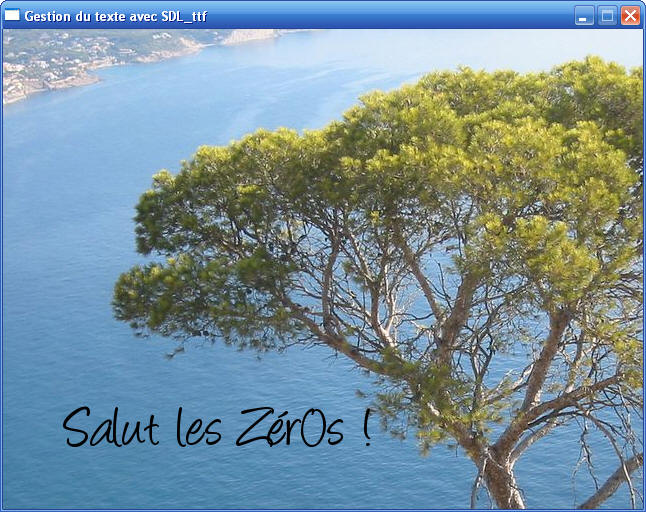
\includegraphics[width=0.6\textwidth]{Chapter_III-7_Blended-text}
\end{figure}

إذا أردت تغيير طريقة الكتابة للتجريب، لا يوجد سوى سطر للتعديل : السطر الخاص بإنشاء المساحة (استدعاء الدالة 
\InlineCode{TTF\_RenderText\_Blended}).

\begin{warning}
تأخذ الدالة
\InlineCode{TTF\_RenderText\_Shaded}
معاملا رابعا على عكس الأخرتين. هذا المعامل الأخير هو لون الخلفية الذي نريد استعماله. يجب عليك إذا إنشاء متغير من نوع
\InlineCode{SDL\_Color}
للإشارة إلى لون الخلفية (مثلا أبيض).
\end{warning}

\subsection{خصائص كتابة نص}

يمكن أيضاً تحديد خصائص الخط، كـغليظ مثلاً، مائل و مسطّر. 

يجب أولاّ أن يتم تحميل الخط و لهذا يجب أن يتوفر لديك متغير
\InlineCode{font}
صحيح. و يمكنك إذا استدعاء الدالة 
\InlineCode{TTF\_SetFontStyle}
التي ستقوم بالتعديل على الخط لكي يكون غليظا، مائلا أو مسطّرا حسب الرغبة. الدالة تأخذ معاملين :

\begin{itemize}
	\item الخط الذي نريد تعديله.
	\item دمج أعلام للإشارة إلى نمط الكتابة الذي نريد إعطاءه : غليظ، مائل أو مسطّر.
\end{itemize}

بالنسبة للأعلام، يجب عليك استعمال الثوابت التالية :

\begin{itemize}
	\item \InlineCode{TTF\_STYLE\_NORMAL} :
	عادي.
	\item \InlineCode{TTF\_STYLE\_BOLD} :
	غليظ.
	\item \InlineCode{TTF\_STYLE\_ITALIC} :
	مائل.
	\item \InlineCode{TTF\_STYLE\_UNDERLINE} :
	مسطّر.
\end{itemize}

بما أنها قائمة من الاعلام، يمكنك الدمج بينها باستعمال الإشارة
\InlineCode{|}
كما تعلّمنا القيام بذلك سابقاً.

فلنجرّب :

\begin{Csource}
// Loading the font
font = TTF_OpenFont("angelina.ttf", 65);
// The text will be italic and underlined
TTF_SetFontStyle(font, TTF_STYLE_ITALIC | TTF_STYLE_UNDERLINE);
// Writing the text in italic and underlined modes
text = TTF_RenderText_Blended(font, "Salut les Zér0s !", blackColor);
\end{Csource}

النتيجة : النص مكتوب بخاصية مائل و مسطّر :

\begin{figure}[H]
	\centering
	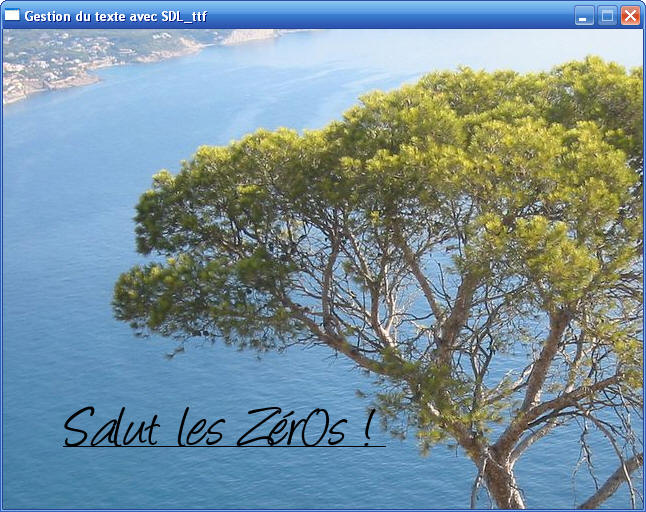
\includegraphics[width=0.6\textwidth]{Chapter_III-7_Italic-underlined-text}
\end{figure}

لإرجاع خط ما إلى حالته العاديّة، يكفي أن نعيد استدعاء الدالة
\InlineCode{TTF\_SetFontStyle}
باستعمال العلم
\InlineCode{TTF\_STYLE\_NORMAL}
هذه المرّة.

\subsection{تمرين : العداد}

سيجمع هذا التمرين بين المفاهيم التي تعلّمتها في هذا الفصل و فصل التحكّم في الوقت. مهمّتك، إن قبلتها، هي إنشاء عداد تتصاعد قيمته كلّ أعشار الثانية، أي أنه سيُظهر بشكل تقدّمي القيم التالية : 0، 100، 200، 300، 400 \dots
بعد ثانية، يجدر بالرقم 1000 أن يظهر.

\subsubsection{طريقة للكتابة في سلسلة محارف}

لكي تحلّ هذا التمرين، ستحتاج إلى معرفة كيفية الكتابة داخل سلسلة محارف في الذاكرة.\\
في الواقع يجب عليك أن تعطي للدالة
\InlineCode{TTF\_RenderText}
متغيرا من نوع
\InlineCode{char*}
لكن ماهو متوفّر لديك هو عدد (من نوع
\InlineCode{int}
مثلا). كيف يمكننا تحويل عدد إلى سلسلة محارف ؟

يمكننا أن نستعمل من أجل هذا الدالة
\InlineCode{sprintf}.\\
إنها تعمل بنفس الطريقة التي تعمل بها
\InlineCode{fprintf}،
الاختلاف الوحيد هو أنه في عوض الكتابة في ملف، ستتم الكتابة في سلسلة محارف (الحرف
\textenglish{s}
يختصر الكلمة
\textenglish{string}
و التي تعني "سلسلة محارف" بالإنجليزيّة).\\
أوّل معامل تقدّمه سيكون إذا مؤشّرا نحو جدول من
\InlineCode{char}.

\begin{critical}
قم بحجز مكان كافٍ من أجل جدول
\InlineCode{char}
إذا أردت ألا تتجاوز في الذاكرة !
\end{critical}

مثال :

\begin{Csource}
sprintf(time, "Temps : %d", counter);
\end{Csource}

هنا، المتغير
\InlineCode{time}
هو جدول محارف (20 محرفا)، و
\InlineCode{counter}
هو متغير من نوع
\InlineCode{int}
يحوي الزمن.\\
بعد هذه التعليمة، سلسلة المحارف 
\InlineCode{time}
ستحتوي مثلا على
"\textenglish{Temps : 500}".

هيّا، حان وقتُ العمل !

\subsection{التصحيح}

هذا تصحيح ممكن للتمرين :

\begin{Csource}
int main(int argc, char *argv[])
{
	SDL_Surface *screen = NULL, *text = NULL;
	SDL_Rect position;
	SDL_Event event;
	TTF_Font *font = NULL;
	SDL_Color blackColor = {0, 0, 0}, whiteColor = {255, 255, 255};
	int cont = 1;
	int currentTime = 0, previousTime = 0, counter = 0;
	char time[20] = ""; // A table of char big enough
	SDL_Init(SDL_INIT_VIDEO);
	TTF_Init();
	screen = SDL_SetVideoMode(640, 480, 32, SDL_HWSURFACE | SDL_DOUBLEBUF);
	SDL_WM_SetCaption("Gestion du texte avec SDL_ttf", NULL);
	// Loading the police
	font = TTF_OpenFont("angelina.ttf", 65);
	// Time and text initialization
	currentTime = SDL_GetTicks();
	sprintf(time, "Temps : %d", counter);
	text = TTF_RenderText_Shaded(font, time, blackColor, whiteColor);
	while (cont)
	{
		SDL_PollEvent(&event);
		switch(event.type)
		{
			case SDL_QUIT:
			cont = 0;
			break;
		}
		SDL_FillRect(screen, NULL, SDL_MapRGB(screen->format, 255, 255, 255));
		currentTime = SDL_GetTicks();
		if (currentTime - previousTime >= 100) // If 100ms at least have passed
		{
			counter += 100; // We add 100ms to the counter
			sprintf(time, "Temps : %d", counter); // We write in the string "time" the new time
			SDL_FreeSurface(text);// We delete the previous surface
			text = TTF_RenderText_Shaded(font, time, blackColor, whiteColor); // We write the sring "time" in SDL_Surface
			previousTime = currentTime; // We update the previous time
		}
		position.x = 180;
		position.y = 210;
		SDL_BlitSurface(text, NULL, screen, &position); // Blitting the text
		SDL_Flip(screen);
	}
	TTF_CloseFont(font);
	TTF_Quit();
	SDL_FreeSurface(text);
	SDL_Quit();
	return EXIT_SUCCESS;
}
\end{Csource}
 
الصورة التالية تمثّل النتيجة في غضون 13,9 ثانية بالتحديد :

\begin{figure}[H]
	\centering
	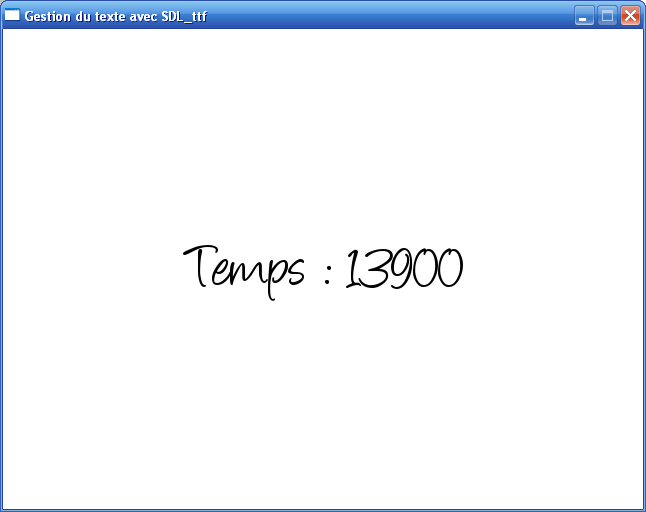
\includegraphics[width=0.6\textwidth]{Chapter_III-7_Time-text}
\end{figure}

لا تتردد في تنزيل المشروع إذا أردت دراسته بالتفصيل و تحسينه. هو ليس مثالياً بعد : يمكننا مثلاً استعمال
\InlineCode{SDL\_Delay}
لتجنّب استعمال المعالج بنسبة 100\%.

\textenglish{\url{https://openclassrooms.com/uploads/fr/ftp/mateo21/ttf_exercice_temps.zip} (437 Ko)}

\subsubsection{للذهاب بعيدا}

إذا أردت التقدّم و تحسين هذا البرنامج، يمكنك أن تحاول صنع لعبة أين يجب النقر بالفأرة العدد الأقصى من المرات الممكنة في النافذة في وقت محدود حيث تتزايد قيمة العداد بعد كلّ نقرة.

يجب أن يتم إظهار عداد عكسي. حينما يصل إلى الصفر، نظهر عدد النقرات التي تم القيام بها و نطلب من المستعمل ما إن كان يريد إعادة المحاولة.

يمكنك أيضاً معالجة أفضل النتائج و تسجيلها في ملف. هذا سيساعدك في التدرب من جديد على استخدام الملفات في الـ\textenglish{C}.

حظاً موفقا !

\section*{ملخّص}

\begin{itemize}
	\item لا يمكننا أن نكتب نصاً في الـ\textenglish{SDL}،
	إلا إن استعملنا تمديداً كالمكتبة 
	\textenglish{SDL\_ttf}.
	\item تسمح هذه المكتبة بتحميل ملفات خطوط ذات صيغة 
	\InlineCode{.ttf}
	بالاستعانة بالدالة
	\InlineCode{TTF\_OpenFont}.
	\item توجد ثلاث طرق لكتابة نص، ترتيبها من الأبسط إلى الأكثر تعقيدا :
	\textenglish{Solid}،
	ثم
	\textenglish{Shaded}
	ثم
	\textenglish{Blended}.
	\item يمكننا الكتابة في
	\InlineCode{SDL\_Surface}
	عن طريق دوال مثل
	\InlineCode{TTF\_RenderText\_Blended}.
\end{itemize}
